%--------------------------------------------------------------------------
\chapter{Conclusion} \label{ch:conclusion}
%--------------------------------------------------------------------------



perception research into laryngeal complexity is lacking

%--------------------------------------------------------------------------
\section{The Laryngeal Articulator Model}\label{sec:lam}
%--------------------------------------------------------------------------

\citet{eslingThereAreNo2005,eslingVoiceQualityLaryngeal2019,moisikPhonologicalPotentialsLower2021,moisikMultimodalImagingGlottal2015,moisikModelingBiomechanicalInfluence2014}

\begin{figure}
    \centering
    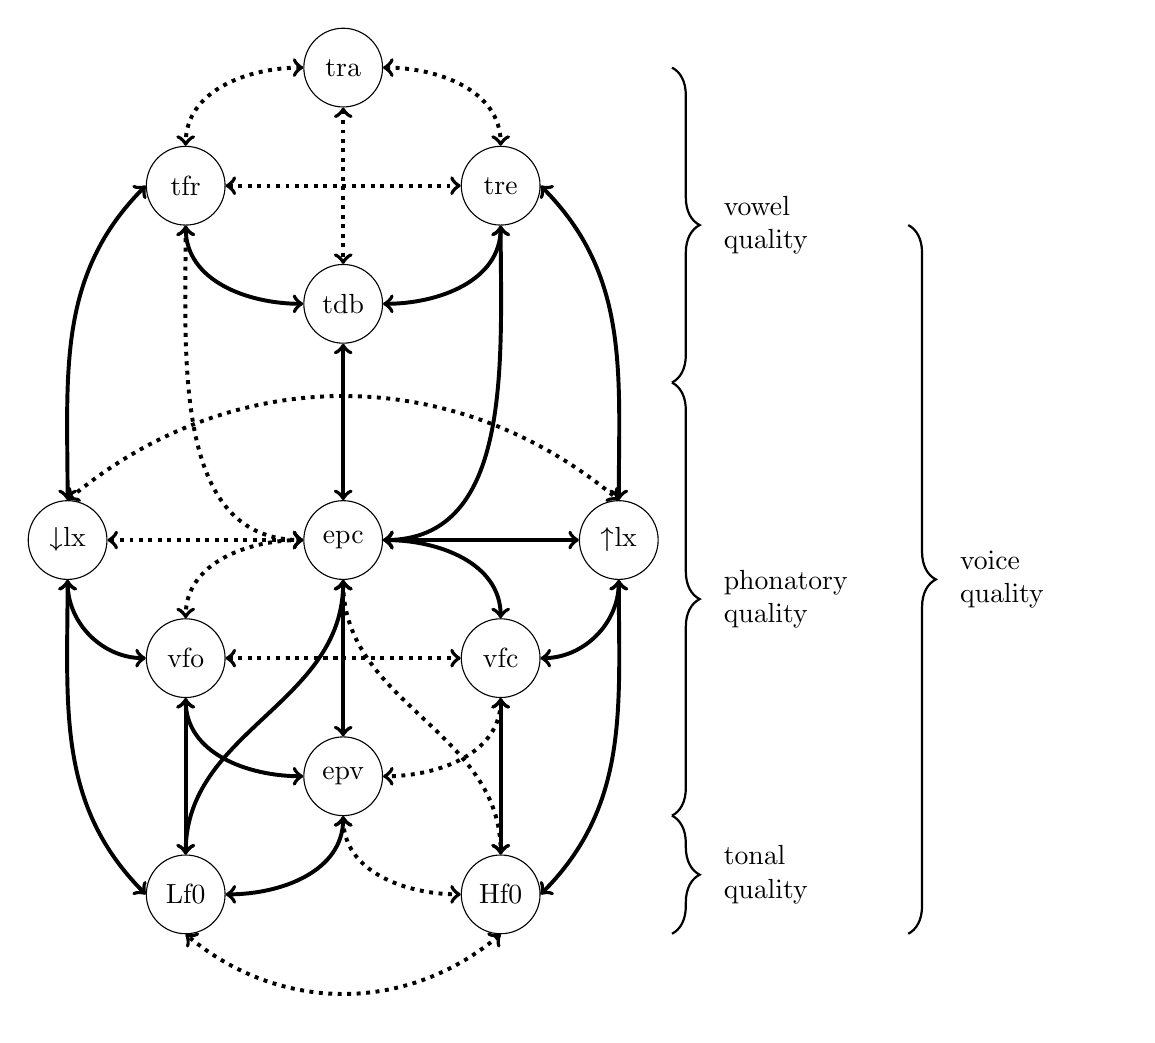
\begin{tikzpicture}
        \node[draw,circle,minimum size=1cm,inner sep=0pt] (tra) at (0,0) {tra};
        \node[draw,circle,minimum size=1cm,inner sep=0pt] (tfr) at (-2,-1.5) {tfr};
        \node[draw,circle,minimum size=1cm,inner sep=0pt] (tre) at (2,-1.5) {tre};
        \node[draw,circle,minimum size=1cm,inner sep=0pt] (tdb) at (0,-3) {tdb};

        \node[draw,circle,minimum size=1cm,inner sep=0pt] (epc) at (0,-6) {epc};
        \node[draw,circle,minimum size=1cm,inner sep=0pt] (vfo) at (-2,-7.5) {vfo};
        \node[draw,circle,minimum size=1cm,inner sep=0pt] (vfc) at (2,-7.5) {vfc};
        \node[draw,circle,minimum size=1cm,inner sep=0pt] (epv) at (0,-9) {epv};

        \node[draw,circle,minimum size=1cm,inner sep=0pt] (lower_lx) at (-3.5,-6) {↓lx};
        \node[draw,circle,minimum size=1cm,inner sep=0pt] (raised_lx) at (3.5,-6) {↑lx};

        \node[draw,circle,minimum size=1cm,inner sep=0pt] (Lf0) at (-2,-10.5) {Lf0};
        \node[draw,circle,minimum size=1cm,inner sep=0pt] (Hf0) at (2,-10.5) {Hf0};
        
        % Anti-syngeristic
        \draw[<->, dotted, line width=.5mm] (tra.west) to[out=180,in=90] (tfr.north);
        \draw[<->,dotted, line width=.5mm] (tra.east) to[out=0,in=90] (tre.north);
        \draw[<->,dotted, line width=.5mm] (tfr.east) to (tre.west);
        \draw[<->,dotted, line width=.5mm] (tra.south) to (tdb.north);
        \draw[<->,dotted, line width=.5mm] (tfr.south) to[in=180, out=-90] (epc.west);
        \draw[<->,dotted, line width=.5mm] (lower_lx.north) to[in=140,out=40] (raised_lx.north);
        \draw[<->,dotted, line width=.5mm] (lower_lx.east) to (epc.west);
        \draw[<->,dotted, line width=.5mm] (epc.west) to[in=90,out=180] (vfo.north);
        \draw[<->,dotted, line width=.5mm] (vfo.east) to[in=180,out=0] (vfc.west);
        \draw[<->,dotted, line width=.5mm] (vfc.south) to[in=0,out=-90] (epv.east);
        \draw[<->,dotted, line width=.5mm] (epc.south) to[out=-90, in=90] (Hf0.north);
        \draw[<->,dotted, line width=.5mm] (Hf0.south) to[out=-140, in=-40] (Lf0.south);
        \draw[<->,dotted, line width=.5mm] (epv.south) to[out=-90, in=180] (Hf0.west);

        % Syngeristic
        \draw[<->, line width=.5mm] (tdb.west) to[out=180, in=-90] (tfr.south);
        \draw[<->, line width=.5mm] (tdb.east) to[out=0, in=-90] (tre.south);
        \draw[<->, line width=.5mm] (epc.north) to (tdb.south);
        \draw[<->, line width=.5mm] (epc.south) to (epv.north);
        \draw[<->, line width=.5mm] (epc.east) to[in=-90, out=0] (tre.south);
        \draw[<->, line width=.5mm] (lower_lx.north) to[in=-135, out=90] (tfr.west);
        \draw[<->, line width=.5mm] (raised_lx.north) to[in=-45, out=90] (tre.east);
        \draw[<->, line width=.5mm] (Lf0.west) to[in=-90, out =135] (lower_lx.south);
        \draw[<->, line width=.5mm] (raised_lx.west) to (epc.east);
        \draw[<->, line width=.5mm] (Hf0.east) to[in=-90, out=45] (raised_lx.south);
        \draw[<->, line width=.5mm] (epv.south) to[out=-90, in=0] (Lf0.east);
        \draw[<->, line width=.5mm] (epc.east) to[out=0, in=90] (vfc.north);
        \draw[<->, line width=.5mm] (vfo.south) to[out=-90, in=180] (epv.west);
        \draw[<->, line width=.5mm] (vfc.south) to (Hf0.north);
        \draw[<->, line width=.5mm] (vfo.south) to (Lf0.north);
        \draw[<->, line width=.5mm] (epc.south) to[out=-90,in=90] (Lf0.north);
        \draw[<->, line width=.5mm] (lower_lx.south) to[out=-90,in=180] (vfo.west);
        \draw[<->, line width=.5mm] (raised_lx.south) to[out=-90,in=0] (vfc.east);

        % Curly bracket with text
        \draw[decorate,decoration={brace,amplitude=10pt,raise=5pt},thick] (4,0) -- (4,-4) node[midway,xshift=15pt,right=5pt] {\parbox{2cm}{vowel\\quality}};
        \draw[decorate,decoration={brace,amplitude=10pt,raise=5pt},thick] (4,-4) -- (4,-9.5) node[midway,xshift=15pt,right=5pt] {\parbox{2cm}{phonatory\\quality}};
        \draw[decorate,decoration={brace,amplitude=10pt,raise=5pt},thick] (4,-9.5) -- (4,-11) node[midway,xshift=15pt,right=5pt] {\parbox{2cm}{tonal\\quality}};
        \draw[decorate,decoration={brace,amplitude=10pt,raise=5pt},thick] (7,-2) -- (7,-11) node[midway,xshift=15pt,right=5pt] {\parbox{2cm}{voice\\quality}};

        
    \end{tikzpicture}
    \caption{The Laryngeal Articulator Model from \citet{eslingVoiceQualityLaryngeal2019}. This model shows the interactions between the laryngeal articulators (labeled circles). Syngeristic interactions are shown with solid lines, while anti-syngeristic interactions are shown with dotted lines.}
    \label{fig:tra}
\end{figure}

%--------------------------------------------------------------------------
\section{Modeling laryngeal complexity}\label{sec:modeling_lc}
%--------------------------------------------------------------------------

%--------------------------------------------------------------------------
\section{Alternative accounts}\label{sec:alternative_accounts}
%--------------------------------------------------------------------------

%--------------------------------------------------------------------------
\subsection{Articulatory Phonology account}\label{sec:ap_account}
%--------------------------------------------------------------------------

%--------------------------------------------------------------------------
\subsection{Q-theory account}\label{sec:q_theory_account}
%--------------------------------------------------------------------------

%--------------------------------------------------------------------------
\subsection{Radical CV Phonology account}\label{sec:rcv_account}
%--------------------------------------------------------------------------

%--------------------------------------------------------------------------
\section{Typological implications}\label{sec:typological_implications}
%--------------------------------------------------------------------------

\begin{itemize}
    \item Another aspect of my research into the tone and phonation interactions is why we see gaps/restrictions for which tones and phonations are allowed to combine. 
    \begin{itemize}
        \item This is important because of the gaps I observe in SLZ where some we never see breathy with high tone and we do not see checked vowels with rising tone. 
        \begin{itemize}
            \item This is true for nominals. 
            \item I have not looked at verbs and whether or not we see this same gap. 
            \begin{itemize}
                \item I expect that the gap is also present in the verbal paradigms similar to what \citet{uchiharaToneRegistrogenesisQuiavini2016} observed where breathy phonation fails to appear in some parts of the paradigm.
                \item Especially with the Potential Aspect, which is always realized as a high tone on the verbal root. 
            \end{itemize}
        \end{itemize}
    \end{itemize}
    \item These four types of languages offer an excellent way for me to characterize what we see cross-linguistically in the interactions between tone and phonation. 
    \item This primarily is useful for me as a way to zero in on which languages I need to look at. 
    \begin{itemize}
        \item This means that I need to focus my search into types IIb, IIIb, and IV languages.
    \end{itemize}
\end{itemize}
